% siminos/atlas/cut.tex  pdflatex atlas
% $Author$ $Date$

\section{Dynamics and symmetries: a recap}
\label{s:cut}

\subsection{Group orbit}


    \ifdraft\color{blue}
%%%%%%%%%%%%%%%%%%%%%%%%%%%%%%%%%%%%%%%%%%%%%%%%%%%%%%%%%%%%%%%%%%%%%
\begin{figure}
   \centering
(a)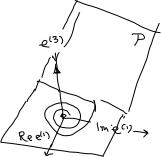
\includegraphics[width=0.20\textwidth]{A29PoincBad}
(b)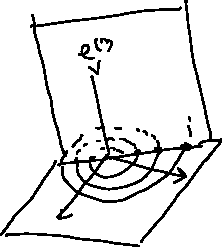
\includegraphics[width=0.20\textwidth]{A29PoincGood}
   \caption{\label{fig:A29PoincBad}
    (a)
Bad section.
    (b)
Good section.
}
\end{figure}
%%%%%%%%%%%%%%%%%%%%%%%%%%%%%%%%%%%%%%%%%%%%%%%%%%%%%%%%%%%%%%%%%%%%%

\refFig{fig:A29PoincBad}\,({\it a}) shows why \reffig{f:RosslSect} is OK for
capturing the strange attractor, but actually bad; the lower \eqv\
$\ssp_{-}$ does not lie on the $z$ axis, so a section that includes the
$z$ axis misses the motions close to  $\ssp_{-}$.

In order to illustrate \PoincBord, we need two charts like
\reffig{fig:robbins3-7} (by Bryce, see robbins3-7.nb), and hopefully ta
sensible combined 2-chart atlas (no one has drown that one). All figures
should be small in size, and laid out like \reffig{f:RosslSect}, with
sensible $z$-axis.
    \PC{2012-03-28~~
    Some pointers to figure drawing are in {siminos/figSrc/00ReadMe.txt}.
    }


%%%%%%%%%%%%%%%%%%%%%%%%%%%%%%%%%%%%%%%%%%%%%%%%%%%%%%%%%%%%%%%%%%%%%
\begin{figure}
   \centering
(a)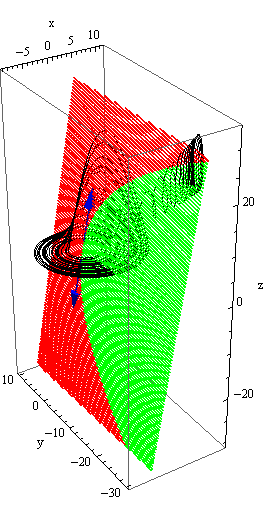
\includegraphics[width=0.16\textwidth]{robbins3-7a}
(b)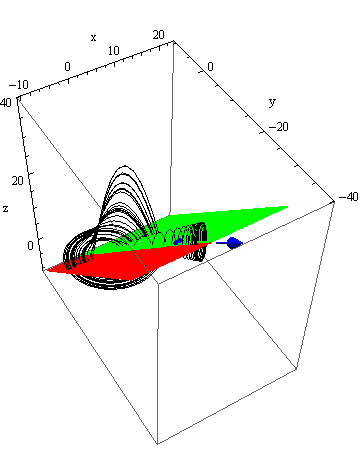
\includegraphics[width=0.24\textwidth]{robbins3-7b}
\\
(c)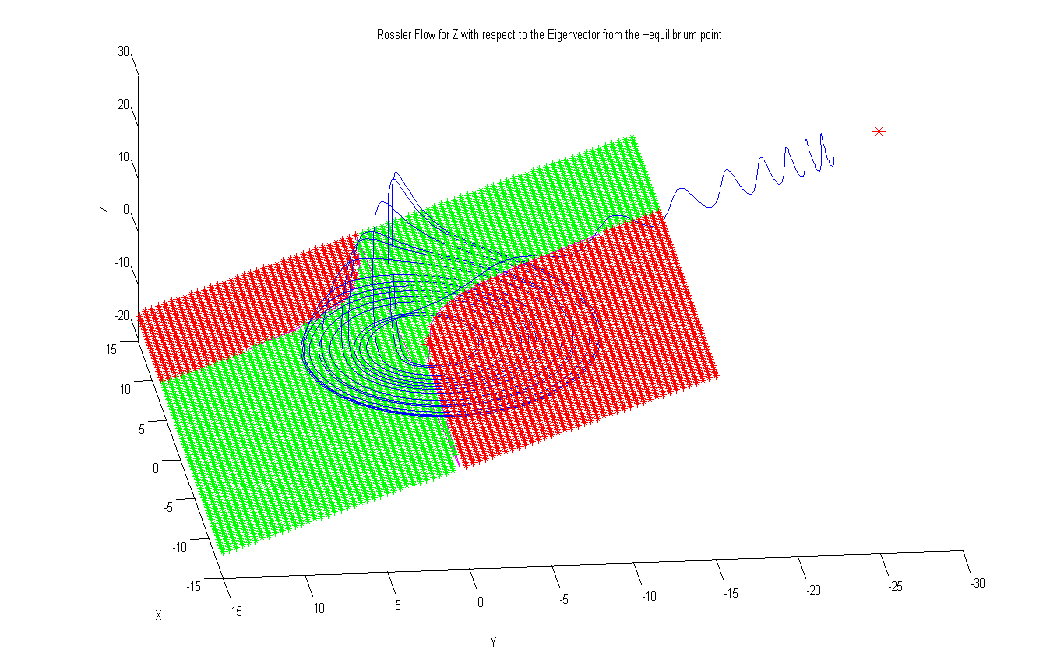
\includegraphics[width=0.44\textwidth]{wadsworth3-7a}
   \caption{\label{fig:robbins3-7}
    (a)
A section as in \refFig{fig:A29PoincBad}\,({\it b}), correctly centered
centered on $\ssp_{-}$ (Robbins).
    (b)
A section centered on $\ssp_{+}$ (Robbins).
    (c)
(Wadsworth).
}
\end{figure}
%%%%%%%%%%%%%%%%%%%%%%%%%%%%%%%%%%%%%%%%%%%%%%%%%%%%%%%%%%%%%%%%%%%%%

%%%%%%%%%%%%%%%%%%%%%%%%%%%%%%%%%%%%%%%%%%%%%%%%%%%%%%%%%%%%%%%%%%%%%
\begin{figure}
   \centering
(a)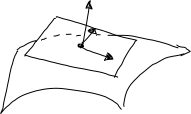
\includegraphics[width=0.20\textwidth]{A27groupTan}
(b)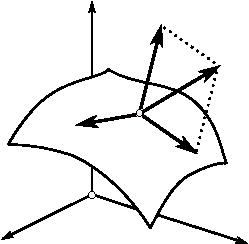
\includegraphics[width=0.20\textwidth]{A28tangents}
   \caption{\label{fig:tangents}
    (a)
A group tangent space at \statesp\ point $\ssp$.
    (b)
In presence of 2-continuous parameter symmetry, each \statesp\ point
$\ssp$ owns 3 tangent vectors: one $\vel(\ssp)$ along the time flow, and
the two group tangents $\groupTan^{(1)}(\ssp)$, $\groupTan^{(2)}(\ssp)$
along infinitesimal symmetry shifts.
}
\end{figure}
%%%%%%%%%%%%%%%%%%%%%%%%%%%%%%%%%%%%%%%%%%%%%%%%%%%%%%%%%%%%%%%%%%%%%

%%%%%%%%%%%%%%%%%%%%%%%%%%%%%%%%%%%%%%%%%%%%%%%%%%%%%%%%%%%%%%%%%%%%%
\begin{figure}
   \centering
(a)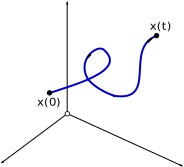
\includegraphics[width=0.20\textwidth]{A27traj}
(b)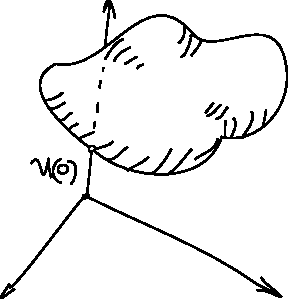
\includegraphics[width=0.20\textwidth]{A27gOrbit}
    \\
(c)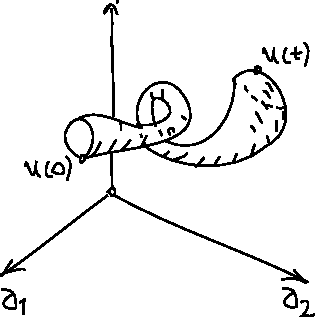
\includegraphics[width=0.20\textwidth]{A27wurst}
   \caption{\label{fig:A27wurst}
    (a)
Trajectory.
    (b)
Group orbit.
    (c)
Wurst.
}
\end{figure}
%%%%%%%%%%%%%%%%%%%%%%%%%%%%%%%%%%%%%%%%%%%%%%%%%%%%%%%%%%%%%%%%%%%%%

%%%%%%%%%%%%%%%%%%%%%%%%%%%%%%%%%%%%%%%%%%%%%%%%%%%%%%%%%%%%%%%%%%%%%
\begin{figure}
   \centering
(a)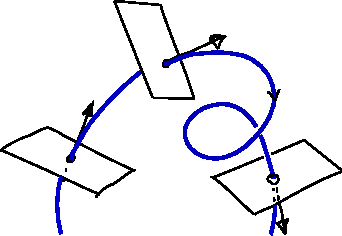
\includegraphics[width=0.20\textwidth]{A28mConnect}
(b)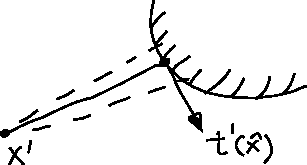
\includegraphics[width=0.20\textwidth]{A28extremum}
   \caption{\label{fig:A28extremum}
    (a)
Method of connections.
    (b)
Extremal condition for nearest distance.
}
\end{figure}
%%%%%%%%%%%%%%%%%%%%%%%%%%%%%%%%%%%%%%%%%%%%%%%%%%%%%%%%%%%%%%%%%%%%%


define
\begin{itemize}
  \item dynamical system $\{\pS,\map^t\}$ with symmetry \Group\
        vs reduced dynamics $\{\pSRed,\mapRed^t\}$
  \item \statesp\ vs tangent space, see \reffig{fig:tangents}
  \item time trajectory \flowRed{\zeit}{\ssp} vs group orbit
        $\pS_\ssp = \{\LieEl\,\ssp \mid \LieEl \in {\Group}\}$
  \item \template
  \item section {\PoincS} vs slice \pSRed
  \item strobing $\sim$ method of connections
  \item reduction vs projection
\end{itemize}
will explain later on

Nature, she don't care :
turbulence breaks all symmetries

{\Large Das Problem}
Drifting is energetically cheap.
Flows are lazy, rather than do work, solutions drift along non-shape-changing
symmetry directions.

    \color{black}\fi

The \emph{group orbit} $\pS_\ssp $ of a \statesp\ point $\ssp \in \pS$ is
traced out by the set of all group actions
\beq
\pS_\ssp = \{\LieEl\,\ssp \mid \LieEl \in {\Group}\}
% \,,\qquad \pS_\ssp \subset \pS
\,.
\ee{sspOrbit}
Any state in the  group orbit set $\pS_{\ssp}$
is physically equivalent to any other. The action of a symmetry group
thus stratifies the \statesp\ into a union of group orbits,
\reffig{fig:BeThTraj}\,{(a)}.

\subsection{Norms - distances between states}

We have seen that in presence of the continuous $\SOn{2}$ symmetry
\reqva\ and \rpo s are 2- and 3-dimensional manifolds of physically
equivalent states. How are we to compare a pair of such states? We shall
do this here by determining the minimal distance between them.

In order to quantify
whether two fluid states are close to or far from each other, one
needs a notion of distance between two points in \statesp, measured
here as
\beq
  \Norm{\ssp-\ssp'}^2  = \braket{\ssp-\ssp'}{\ssp-\ssp'} =
\frac{1}{V}
\int_\bCell \! d \bx \;
(\vec{u}-\vec{u}') \cdot (\vec{u}-\vec{u}')
\,,
\ee{innerproduct}
invariant under all symmetries of the flow,
$\Norm{\ssp-\LieEl\,\slicep}=\Norm{\sspRed-\slicep}$
There is no compelling reason to use this {`energy norm'}, other than
that velocity fields is what is generated in a numerical
computation. What norm one actually uses depends very much on the
application; the importance (and arbitrariness) of the choice of
norm cannot be overemphasized. For example, in the study of `optimal perturbations' that
move a laminar solution to a turbulent one, both energy
\citep{TeHaHe10} and dissipation \citep{LoCaCoPeGo11} norms have been
used.
For experimental data sets, pattern recognition type norms could be the
only practical option\rf{MakeThisUp}.
In our quest for \reqva\ and \rpo s\rf{ACHKW11} we
find it advantageous to use a `compensatory' norm \refeq{compensNorm}
that enhances the weight of cross-stream velocities.


\subsection{\Statesp\ visualization}

On perils of thinking linearly: bases such as Fourier modes are
perfectly natural for problems such a bifurcation of a steady state, and
other weak perturbations. They are absolutely unnatural for strongly
nonlinear problems, with many Fourier modes of comparable magnitude and
strongly entangled.

\subsection{\CLe}
\subsection{Experimentalist description: a video 1D to 3D arrays of pixels}
\subsection{Theorist description: $\infty$-\dmn\ \statesp}
\subsection{Time orbit: point is a point, line is a line in all dimensions}
\label{sect:TimeOrb}

\subsection{Physical dimension: covariant Lyapunov vectors}

\section{Poincar\'e sections}
\label{s:cut}

In general there are two strategies for replacing a continuous-time flow
by iterated mappings; by cutting it by Poincar\'e sections, or by
\emph{strobing} it at a sequence of instants in time. While
`strobing' is what any numerical integrator does, by representing a
trajectory by a sequence of time-integration step separated points,
strobing is in general not a reduction of a flow, as the sequence of
strobed points still resides in the full \statesp\ $\pS$, of
dimensionality $d$.

In the {\em Poincar\'e section method} one records the coordinates of a
trajectory whenever the trajectory reaches a
triggering event. A Poincar\'e section (or, from now on,
just a `section') is {\em not} a projection onto a lower-dimensional space:
Rather, it is a local change of coordinates to a direction along the
flow, and the remaining coordinates (spanning the section) transverse to
it. No information about the flow is lost; the full
space trajectory can always be reconstructed by integration from the
nearest point in the section.

    \ifdraft\color{blue}
        There is always tension between mathematics - linear problem eigenmodes
        (Fourier for translations and rotations) and physics - the fact that
        nonlinear dynamics states are far away from such axes, as they
        always involve a number of such linear modes strongly entangled.
    \color{black}\fi


After some experimentation and observations of chaos in a given
flow, one can identify a set of dynamically important unstable
{\recurrStr s}.
We shall refer to this catalogue of $M$ representative snapshots or
`reference states', either precomputed or experimentally measured, as
\emph{\template s}\rf{rowley_reconstruction_2000}, each an
instantaneous state of the $3D$ fluid flow represented by a \emph{point}
$\slicep{}^{(j)}$, $j=1,2,\cdots,M$, in the \statesp\ $\pS$ of the
system.


\subsection{R\"ossler {\poincBord}}

As an example let of take the classic system of R\"ossler\rf{ross}

\index{R\"ossler system}
\beq
\begin{split}
  \dot{x} &= -x \,-\,z \\
  \dot{y} &= x + a y \\
  \dot{z} &= b + z (x - c)
  \label{eq:Rossler}
\end{split}
\eeq

where $a = b = 0.2$ and $c = 5.7$.

%%%%%%%%%%%%%%%%%%%%%%%%%%%%%%%%%%%%%%%%%%%%%%%%%%%%%%%%%%%%%%%%%%%%%
\begin{figure}
   \centering
   %\includegraphics[width=0.45
\begin{minipage}[b]{0.19\textwidth} %{0.39\textwidth}
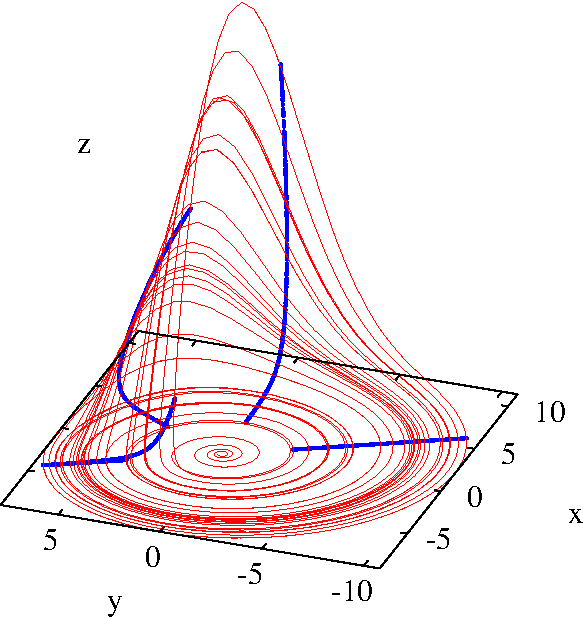
\includegraphics[width=1.15\textwidth,origin=c]
            {Rossler_PsectionB}
\\
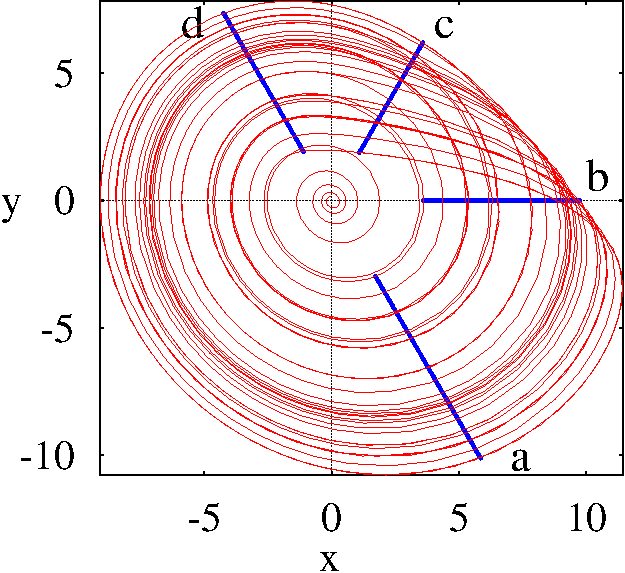
\includegraphics[width=0.80\textwidth,origin=c]
            {Rossler_PsectionA}
  \end{minipage}~~~~~%
  \begin{minipage}[b]{0.25\textwidth} %{0.50\textwidth}
    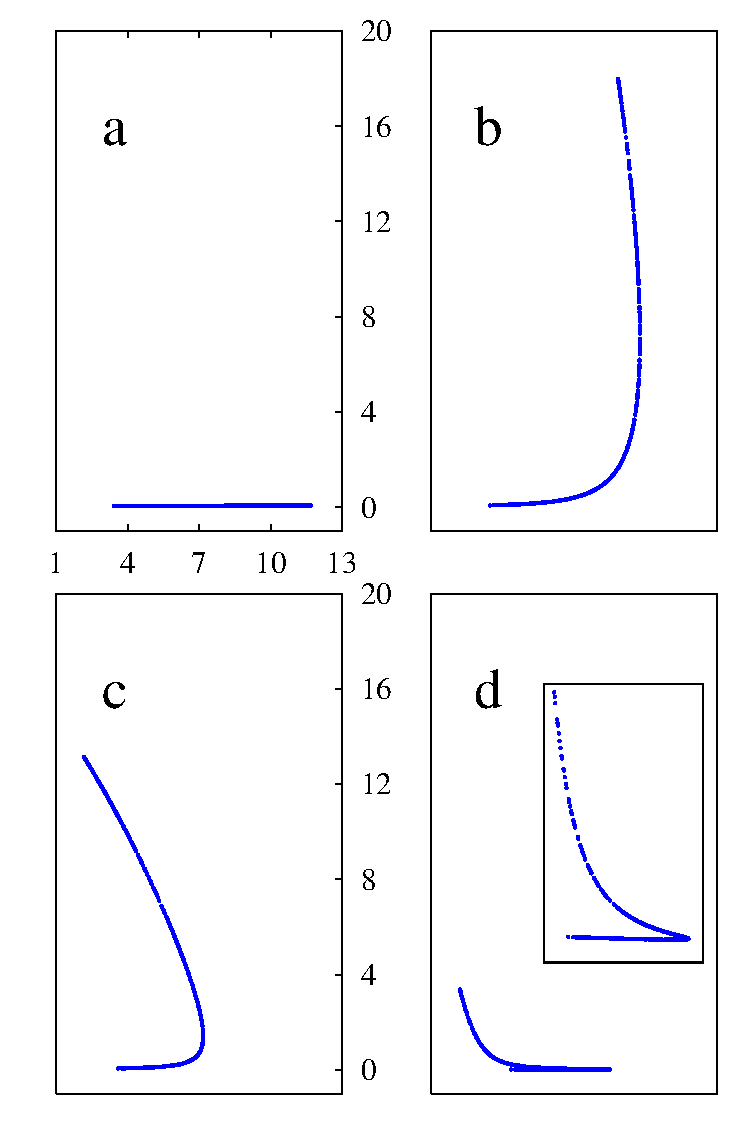
\includegraphics[width=1.00\textwidth]
            {Rossler_PsectionC}
  \end{minipage}
   \caption{\label{f:RosslSect}
      (Right:) a sequence of Poincar\'e sections of
      the R\"ossler strange attractor,
      defined by planes through the $z$~axis, oriented at angles
      (a) $-60^o$
      (b) $0^o$,
      (c) $60^o$,
      (d) $120^o$,
      in the $x$-$y$~plane.
      (Left:) side and $x$-$y$~plane view of a typical trajectory  with
      Poincar\'e sections superimposed.
      (R. Pa\v skauskas)
            }
\end{figure}
%%%%%%%%%%%%%%%%%%%%%%%%%%%%%%%%%%%%%%%%%%%%%%%%%%%%%%%%%%%%%%%%%%%%%

\subsection{R\"ossler two-chart atlas}
\subsection{R\"ossler unstable manifold curvilinear distance}
\subsection{R\"ossler return map}
\subsection{$N$-chart atlas, forward maps}
% \subsection{Ring of Fire return map\rf{lanCvit07}}
